\chapter{VMware Installation and Simulator Guide}

\section{System Requirements}

\begin{itemize}
    \item CPU: i3 desktop or equivalent/ i5 laptop or equivalent
    \item GPU: Integrated Graphics Unit/ Dedicated GPU
    \item Memory: 6G or above
    \item Disk Space: 20G or above
\end{itemize}

Reference Laptop:
\begin{itemize}
    \item CPU: i5 8th Gen
    \item GPU: Intel UHD Graphics 620
    \item Memory: 8G
    \item Disk Space: 20G
\end{itemize}

Note: Simulators are demanding software to run. If you have problems running the virtual machine and/or the simulator, please let the TAs know about your situation. If you believe that it is due to hardware limitations, please check out the technology loan program \url{https://answers.uillinois.edu/illinois/99680}.

\newpage

\section{VMware Installation}

The UIUC WebStore offers free VMware products under VMware Academic Program. \url{https://e5.onthehub.com/WebStore/Welcome.aspx?ws=6c313875-25d6-e311-93fd-b8ca3a5db7a3}\\

Follow the instructions and download VMware Workstation 15.x Player on Windows/Linux or VMware Fusion 11.x Pro for Mac. Note that the guide is only written for VMware Workstation 15.x but not on VMware Fusion 11.x Pro. Please let the instructors know if you experience issues with Mac.

\section{VMware Image}

VMware uses VM image files to run the operating system as well as store files. Please unzip the ECE470VM.zip file and extract it to a working directory. In VMware, click “Open a Virtual Machine” and navigate to your working directory.

\begin{figure}[ht]
	\centering
		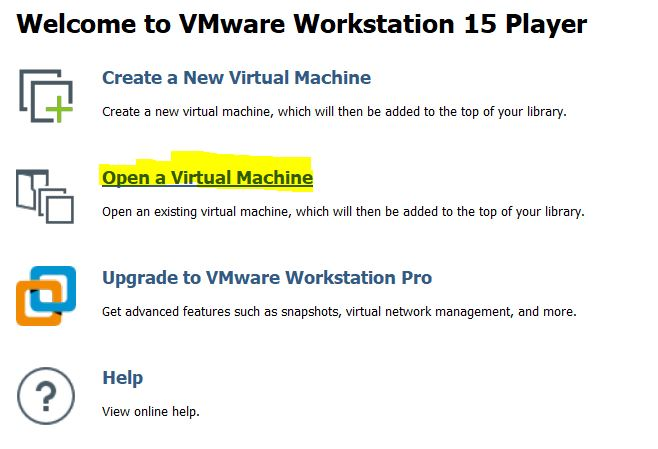
\includegraphics{image/appendixD_vm_open.JPG}
	\caption{Open a Virtual Machine}
\end{figure}

Double click the “ECE470VM.vmx” and you will see the “ECE470VM” option on the left side.

\begin{figure}[ht]
	\centering
		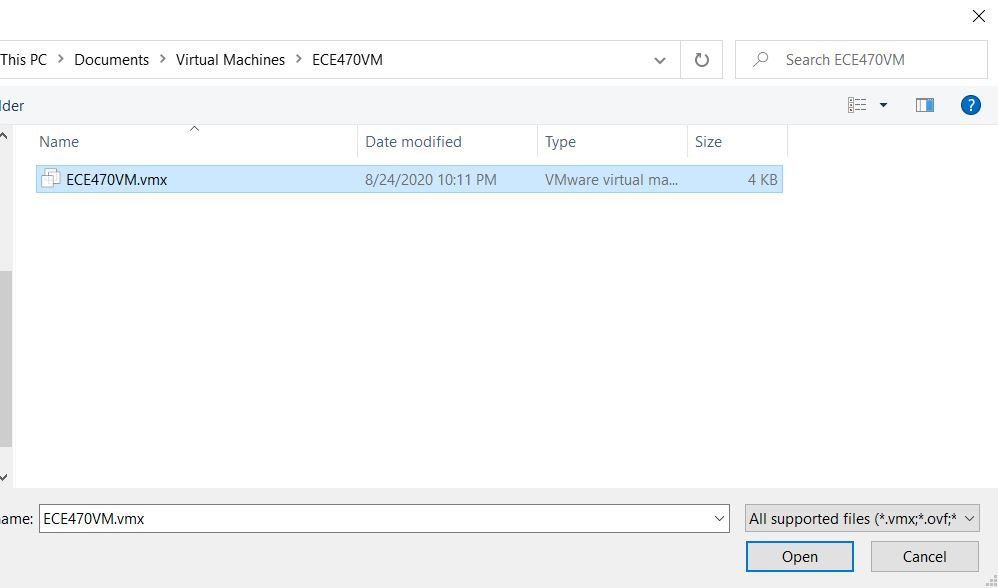
\includegraphics[scale=0.6]{image/appendixD_vm_open_2.JPG}
	\caption{Open vmx file}
\end{figure}

For memory, you need at least 4 GB to run the simulation. Because the host system also requires memory to run, the requirement for memory is at least 6 GB. If your computer has less than 6 GB memory, you need to contact the TAs and use the technology loan program.\\

Now you are ready to boot the system. Click “Play virtual machine” to boot the system. In the new box that asks about whether you moved or copied the virtual machine, choose "I Copied It".

\begin{figure}[ht]
	\centering
		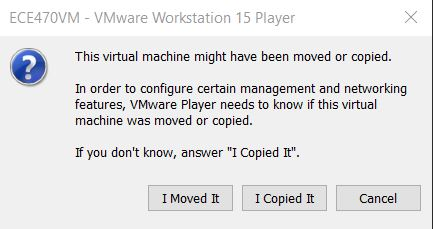
\includegraphics{image/appendixD_vm_copy.JPG}
	\caption{Click "I Copied It"}
\end{figure}

\section{Test}

In the lab, we are mainly going to use two software. To test their functionalities, open a terminal by the shortcut "Ctrl + Alt + T" or other way you prefer. In the terminal window, type in the following command:

\begin{lstlisting}[language=bash]
  $ roscore
\end{lstlisting}

The terminal should print out something similar to this:

\begin{figure}[ht]
	\centering
		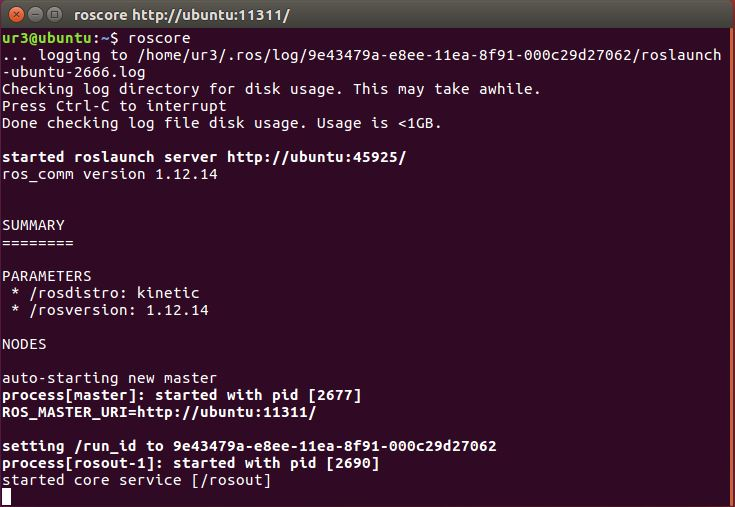
\includegraphics[scale=0.8]{image/appendixD_roscore.JPG}
	\caption{Result of Running "roscore"}
\end{figure}

Now you've tested basic functionalities of ROS, close the ROS core by "Ctrl + C". After the process ends, type in the following command:

\begin{lstlisting}[language=bash]
  $ gazebo
\end{lstlisting}

A new window should pop up and display something like this. If it somehow fails, try running it again. Let the TA know if Gazebo fails consistently. Similarly, after testing, close Gazebo by "Ctrl + C" in the terminal (not the new simulator window).

\begin{figure}[ht]
	\centering
		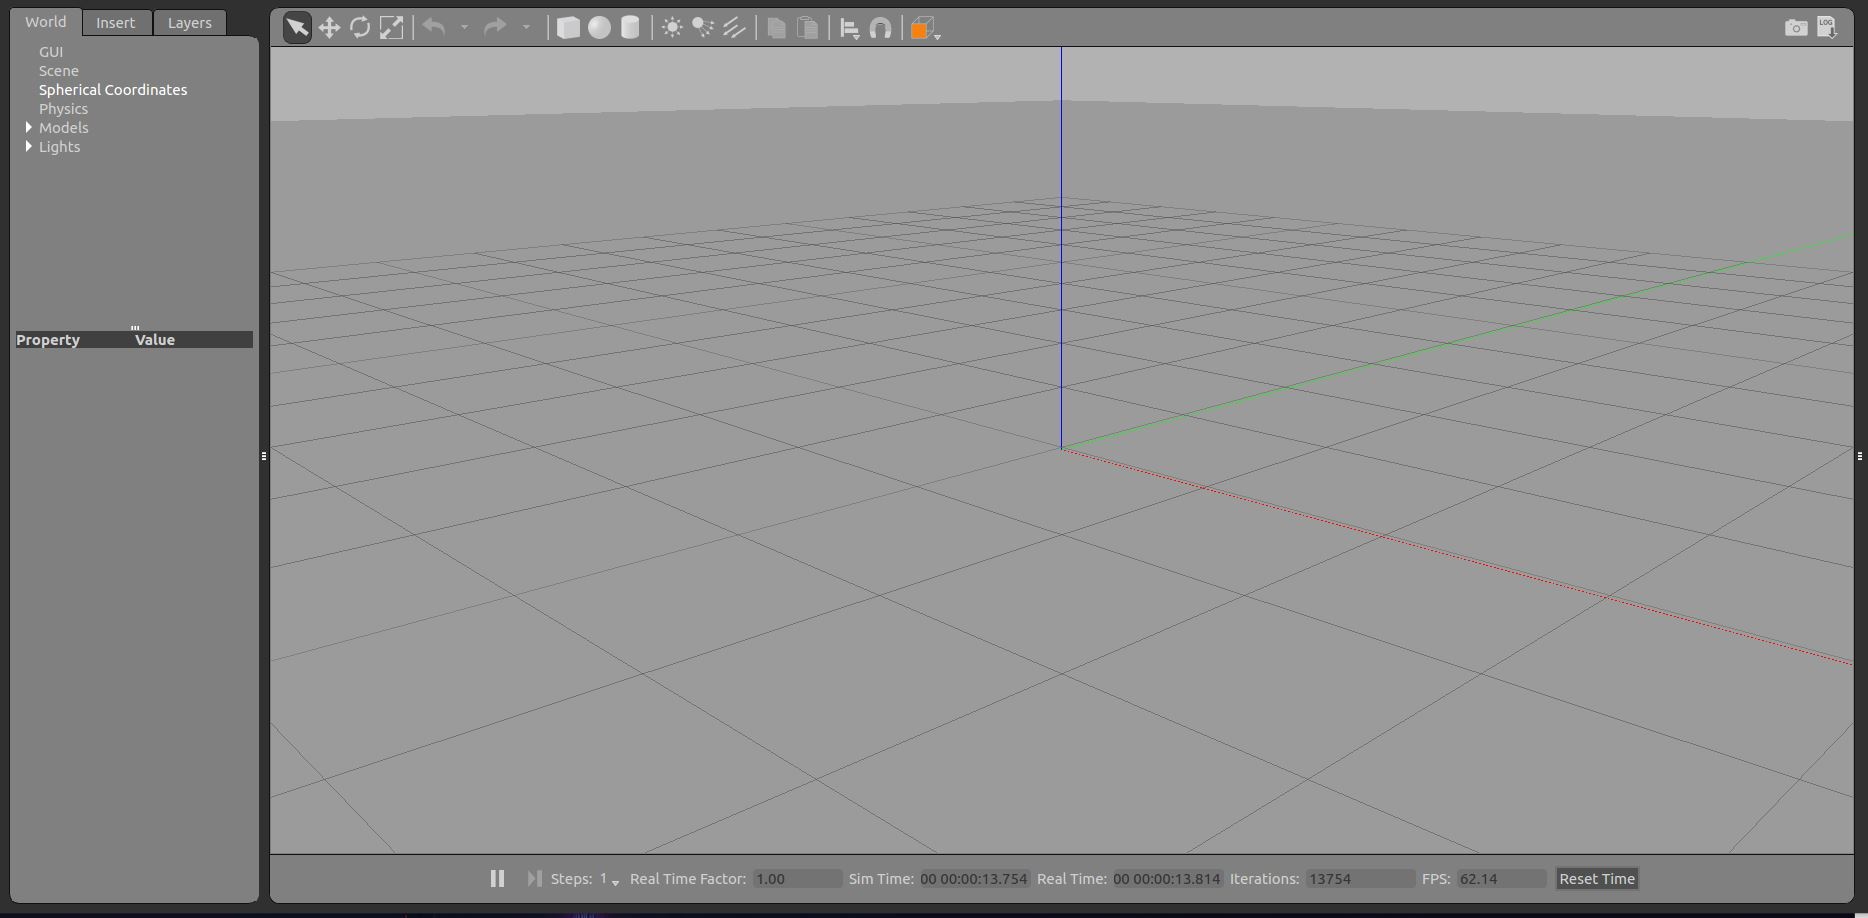
\includegraphics[scale=0.3]{image/appendixD_gazebo.JPG}
	\caption{Result of Running "gazebo"}
\end{figure}


